\documentclass[aspectratio=169]{beamer}

% ---- Theme ----
\usetheme{Singapore}
\usefonttheme{serif}
\usefonttheme[onlylarge]{structurebold}

\setbeamertemplate{navigation symbols}{}
\setbeamertemplate{caption}[numbered]
\setbeamerfont*{frametitle}{size=\normalsize,series=\bfseries}
\setbeamerfont*{framesubtitle}{size=\small}
\setbeamertemplate{section in toc}[sections numbered]

\definecolor{GICBlue}{RGB}{28,78,128}
\definecolor{GICGreen}{RGB}{35,125,95}
\definecolor{GICRed}{RGB}{170,55,55}
\definecolor{GICGray}{RGB}{80,80,80}

\setbeamercolor{structure}{fg=GICBlue}
\setbeamercolor{alerted text}{fg=GICRed}
\setbeamercolor{example text}{fg=GICGreen}
\setbeamercolor{block title}{fg=white,bg=GICBlue}
\setbeamercolor{block body}{fg=black,bg=GICBlue!7}
\setbeamercolor{exampleblock title}{fg=white,bg=GICGreen}
\setbeamercolor{exampleblock body}{fg=black,bg=GICGreen!7}
\setbeamercolor{alertblock title}{fg=white,bg=GICRed}
\setbeamercolor{alertblock body}{fg=black,bg=GICRed!7}

% ---- Packages ----
\usepackage[english]{babel}
\usepackage[utf8]{inputenc}
\usepackage[T1]{fontenc}
\usepackage{amsmath, amssymb}
\usepackage{graphicx}
\usepackage{booktabs}
\usepackage{array}
\usepackage{xcolor}
\usepackage{tikz}
\usepackage{pgfplots}
\pgfplotsset{compat=1.18}
\usetikzlibrary{arrows.meta, positioning, shapes.geometric, calc}

% ---- Macros ----
\newcommand{\done}{\textcolor{GICGreen}{\checkmark}}
\newcommand{\notdone}{\textcolor{GICRed}{$\circ$}}
\newcommand{\dBdtH}{|dB/dt_H|}

\tikzset{
  data/.style={rectangle, rounded corners, draw=GICBlue, fill=GICBlue!8,
    thick, minimum height=8mm, align=center, font=\small},
  proc/.style={rectangle, rounded corners, draw=GICGreen, fill=GICGreen!8,
    thick, minimum height=8mm, align=center, font=\small},
  warn/.style={rectangle, rounded corners, draw=GICRed, fill=GICRed!8,
    thick, minimum height=8mm, align=center, font=\small},
  arrow/.style={-{Latex[length=2mm]}, thick, draw=GICGray}
}

% ---- Metadata ----
\title[Geomagnetic Hazard Forecasting]{Physics-Informed Machine Learning for\\
Regional Geomagnetic Hazard Forecasting}
\subtitle{Milestone~3 Progress Report}
\author{R.~Scotty Rogers\\ \small Group~6 --- Solo Project}
\institute{DSC 288 --- Capstone}
\date{Spring 2026}

% ============================================================
\begin{document}

% ---- SLIDE 1: Title ----
\begin{frame}
  \titlepage
  \vspace{-0.8em}
  \begin{center}
    \small One-hour-ahead station-level $\dBdtH$ threshold exceedance forecasting\\
    Stations: ABK, MEA, SOD, YKC
  \end{center}
\end{frame}
% Speaker notes:
% "Hi, I'm Scotty Rogers, Group 6, working solo. This project builds a
% leakage-safe ML pipeline for one-hour-ahead geomagnetic hazard
% forecasting at four high-latitude ground stations."

% ============================================================
\section{Background}
% ============================================================

% ---- SLIDE 2: Problem Statement ----
\begin{frame}{Problem Statement}
\begin{block}{Why this matters}
Rapid geomagnetic field changes induce hazardous currents (GICs) in power
grids and pipelines. Existing operational forecasts use global indices
(Kp, Dst) that do not resolve \emph{where} on the ground damage risk is
highest.
\end{block}

\begin{block}{Forecasting objective}
Predict whether station-level $\dBdtH$ exceeds a hazard threshold
\alert{one hour ahead} using multimodal Sun-to-ground observations.
\end{block}

\begin{itemize}
  \item Binary classification:
    $y_{s,\,t+60}
      = \mathbb{1}\!\left[\dBdtH(s,\,t{+}60)\;\geq\;\tau_s\right]$
  \item Station-specific models, trained separately for ABK, MEA, SOD, YKC
  \item Output: calibrated probability + binary alert at HSS-optimal threshold
  \item Leakage rule: features at time $t$ use \alert{only} data
        observed at or before $t$
\end{itemize}

\vspace{0.3em}
{\scriptsize\textcolor{GICGray}{Addresses M1 feedback:
  station-specific modeling stated explicitly.}}
\end{frame}
% Speaker notes:
% "The task is binary classification at each station. Models are trained
% separately---this directly addresses Milestone 1 feedback."

% ============================================================
\section{Literature Survey}
% ============================================================

% ---- SLIDE 3: Literature + Gap ----
\begin{frame}{Literature Survey and Project Positioning}
\small
\begin{tabular}{p{0.21\linewidth} p{0.24\linewidth} p{0.22\linewidth} p{0.22\linewidth}}
\toprule
\textbf{Study} & \textbf{Method} & \textbf{Scope} & \textbf{Limitation} \\
\midrule
Camporeale+ 2020 & Gray-box + boosted tree & 3-station $|dB/dt|$ & OMNI + Geospace only \\
Chen+ 2025 & Deep Gaussian Process & Global $dB_H$ & Single-source, no stations \\
Billcliff+ 2026 & SW ensemble + logistic reg. & Global storm index & No regional output \\
Camporeale+ 2025 & Forecast verification & NOAA flare forecasts & Documents calibration failures \\
\bottomrule
\end{tabular}

\vspace{0.6em}
\begin{exampleblock}{Gaps this project addresses}
\begin{enumerate}
  \item Multimodal fusion breadth: 5 source layers (Solar / L1 / GEO / LEO / Ground)
  \item Station-specific $|dB/dt|$ targeting rather than global indices
  \item 2015--2024 coverage spanning active and quiet solar periods
  \item Leakage-safe pipeline engineering + rigorous evaluation protocol
\end{enumerate}
\end{exampleblock}

\vspace{0.3em}
{\scriptsize\textcolor{GICGray}{Addresses M1 feedback:
  novelty is data-fusion breadth and engineering rigor, not a new algorithm.}}
\end{frame}
% Speaker notes:
% "Prior work uses single-source or simulation-assisted features. The novelty
% here is in multimodal data fusion and leakage-safe engineering, not a new
% model architecture."

% ============================================================
\section{Dataset}
% ============================================================

% ---- SLIDE 4: Data Sources ----
\begin{frame}{Sun-to-Ground Data Sources}
\begin{center}
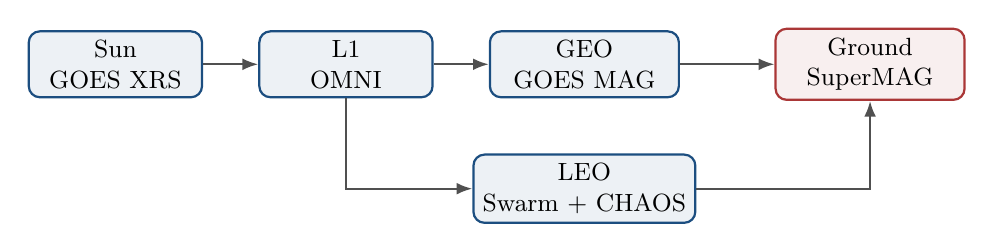
\begin{tikzpicture}[node distance=7mm and 7mm]
  \node[data, minimum width=2.2cm] (sun) {Sun\\GOES XRS};
  \node[data, right=of sun, minimum width=2.2cm] (l1) {L1\\OMNI};
  \node[data, right=of l1, minimum width=2.4cm] (geo) {GEO\\GOES MAG};
  \node[data, below=of geo, minimum width=2.4cm] (leo) {LEO\\Swarm + CHAOS};
  \node[warn, right=12mm of geo, minimum width=2.4cm] (ground)
    {Ground\\SuperMAG};
  \draw[arrow] (sun) -- (l1);
  \draw[arrow] (l1) -- (geo);
  \draw[arrow] (l1) |- (leo);
  \draw[arrow] (geo) -- (ground);
  \draw[arrow] (leo) -| (ground);
\end{tikzpicture}
\end{center}

\small
\begin{tabular}{p{0.12\linewidth} p{0.18\linewidth} p{0.38\linewidth}
  p{0.08\linewidth} p{0.08\linewidth}}
\toprule
\textbf{Layer} & \textbf{Source} & \textbf{Role} & \textbf{Cadence} & \textbf{Status} \\
\midrule
Solar  & GOES XRS     & X-ray flux context / flare driver       & 1\,min & \done \\
L1     & OMNI         & Solar wind + IMF; coupling functions     & 1\,min & \done \\
GEO    & GOES MAG     & Geostationary magnetic-field context     & 1\,min & \done \\
LEO    & Swarm+CHAOS  & Low-Earth-orbit residuals                & 1\,min & \done \\
Ground & SuperMAG     & Target $|dB/dt|$ at ABK/MEA/SOD/YKC     & 1\,min & \done \\
\bottomrule
\end{tabular}

\vspace{0.3em}
Coverage: Jan~2015 -- Dec~2024 (Solar Cycles 24--25).
All 5 source pipelines: download $\to$ clean $\to$ preprocess \done
\end{frame}
% Speaker notes:
% "Five layers trace the full Sun-to-ground chain. All five have complete
% download, cleaning, and preprocessing scripts. Coverage spans 10 years."

% ============================================================
\section{Feature Extraction}
% ============================================================

% ---- SLIDE 5: Pipeline Architecture ----
\begin{frame}{Data Pipeline Architecture}
\begin{center}
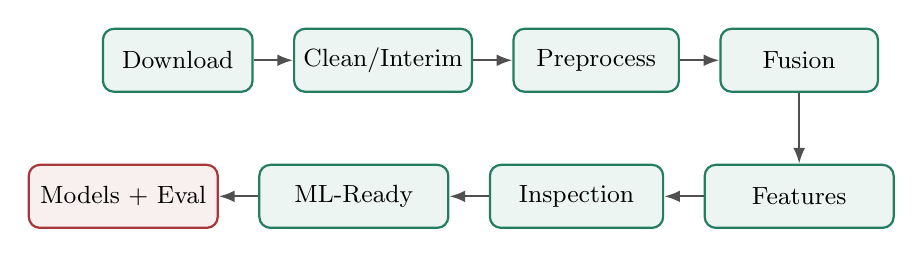
\begin{tikzpicture}[node distance=7mm and 5mm]
  \node[proc, minimum width=1.9cm] (raw) {Download};
  \node[proc, right=of raw,   minimum width=1.9cm] (clean) {Clean/Interim};
  \node[proc, right=of clean, minimum width=2.1cm] (pre) {Preprocess};
  \node[proc, right=of pre,   minimum width=2.0cm] (fuse) {Fusion};
  \node[proc, below=9mm of fuse, minimum width=2.4cm] (feat) {Features};
  \node[proc, left=of feat,  minimum width=2.2cm] (insp) {Inspection};
  \node[proc, left=of insp,  minimum width=2.4cm] (mlr)  {ML-Ready};
  \node[warn, left=of mlr,   minimum width=2.4cm] (mod)  {Models + Eval};

  \draw[arrow] (raw) -- (clean);
  \draw[arrow] (clean) -- (pre);
  \draw[arrow] (pre) -- (fuse);
  \draw[arrow] (fuse) -- (feat);
  \draw[arrow] (feat) -- (insp);
  \draw[arrow] (insp) -- (mlr);
  \draw[arrow] (mlr) -- (mod);
\end{tikzpicture}
\end{center}

\vspace{0.3em}
\small
\begin{tabular}{p{0.38\linewidth} c p{0.40\linewidth}}
\toprule
\textbf{Stage} & \textbf{Status} & \textbf{Key output} \\
\midrule
Download (5 sources)             & \done & \texttt{data/raw/} \\
Clean/Interim (5 sources)        & \done & \texttt{data/interim/} \\
Source-level EDA (5 sources)     & \done & \texttt{data/figures/eda/interim/} \\
Preprocess (6 scripts)           & \done & \texttt{data/preprocessed/} \\
Time-safe Fusion                 & \done & 81 columns, station-time master \\
Feature Engineering              & \done & 268 features + targets \\
Feature Inspection + Leakage     & \done & Audit report: 5/5 checks pass \\
ML-Ready Dataset Builder         & \done & train/val/test parquet + metadata \\
Model Training + Evaluation      & \notdone & Scripts designed, not yet trained \\
\bottomrule
\end{tabular}
\end{frame}
% Speaker notes:
% "Every stage of the pipeline is implemented as a CLI script.
% The entire chain demonstrated end-to-end on January 2015."

% ---- SLIDE 6: EDA Findings ----
\begin{frame}{EDA: Key Findings That Drove Modeling Decisions}
\small
\begin{columns}[T,totalwidth=\textwidth]
\column{0.48\textwidth}
\begin{block}{Target distribution}
\begin{itemize}
  \item $|dB/dt|$ is extremely right-skewed
  \item Mean: 2.71 nT/min, P95: 10.27 nT/min
  \item Event rate (Jan 2015): $\sim$32\%
  \item Confirms binary classification with
        threshold-tuned HSS is appropriate
\end{itemize}
\end{block}

\begin{block}{Station variability}
\begin{itemize}
  \item Event rates differ by station
  \item Supports training separate per-station models
\end{itemize}
\end{block}

\column{0.48\textwidth}
\begin{block}{Missingness structure}
\begin{itemize}
  \item OMNI: 23.2\% missing (gaps during handovers)
  \item GOES XRS/MAG: $<$0.2\% missing
  \item Swarm: 0\% missing (for processed passes)
  \item SuperMAG: $<$0.001\% missing
  \item Structured gaps $\Rightarrow$ missingness-as-signal features
\end{itemize}
\end{block}

\begin{block}{Temporal clustering}
\begin{itemize}
  \item Events cluster in 2015--2018, 2023--2024 (solar maxima)
  \item Chronological split avoids quiet-time leakage
\end{itemize}
\end{block}
\end{columns}
\end{frame}
% Speaker notes:
% "Key EDA findings directly drove modeling decisions: extreme skew confirms
% threshold-based classification, missingness is treated as informative signal,
% and station-level variability supports separate models."

% ---- SLIDE 7: Feature Engineering ----
\begin{frame}{Feature Engineering: 268 Features, 14 Categories}
\scriptsize
\begin{tabular}{p{0.17\linewidth} p{0.20\linewidth} p{0.13\linewidth} p{0.33\linewidth} p{0.06\linewidth}}
\toprule
\textbf{Feature} & \textbf{Source} & \textbf{Lag/Window} &
  \textbf{Physical reason} & \textbf{@\,$t$?} \\
\midrule
\texttt{bz\_gsm\_lag\_60m}    & OMNI      & 60\,min lag   & Southward IMF drives reconnection     & Yes \\
\texttt{newell\_phi}          & OMNI      & instantaneous & SW--magnetosphere coupling rate        & Yes \\
\texttt{speed\_rollmean\_30m} & OMNI      & 30\,min roll  & Sustained solar-wind driving           & Yes \\
\texttt{xrsa\_flux\_lag\_10m} & GOES XRS  & 10\,min lag   & Solar flare context                    & Yes \\
\texttt{gic\_proxy\_lag\_1m}  & SuperMAG  & 1\,min lag    & Recent ground state (persistence info) & Yes \\
\texttt{hour\_sin / hour\_cos}& Derived   & ---           & Diurnal ionospheric conductance        & Yes \\
\texttt{omni\_missing}        & Flag      & instantaneous & Data-quality as signal                 & Yes \\
\texttt{y\_event\_t\_plus\_60}& SuperMAG  & $+$60\,min    & \alert{TARGET --- never in features}   & No  \\
\bottomrule
\end{tabular}

\vspace{0.5em}
\normalsize
\begin{alertblock}{Lead-time rule}
Features at time $t$ use \textbf{only} data observed at or before $t$.
Labels are constructed by station-wise forward shift to $t{+}60$.
No centered rolling windows. Leakage audit: 5/5 checks \textbf{pass}.
\end{alertblock}

\vspace{0.2em}
{\scriptsize\textcolor{GICGray}{Addresses M2 feedback:
  feature table with source, lag/window, physical reason, prediction-time availability.
  Lead-time wording explicit.}}
\end{frame}
% Speaker notes:
% "Every feature is strictly past-facing. The leakage audit
% programmatically verifies this. The target is forward-shifted and never
% enters the feature vector."

% ---- SLIDE 8: Output Schema ----
\begin{frame}{Output Schema: ML-Ready Dataset}
\small
\begin{tabular}{p{0.30\linewidth} p{0.40\linewidth} r}
\toprule
\textbf{Column group} & \textbf{Examples} & \textbf{Count} \\
\midrule
Keys                    & \texttt{timestamp, target\_time, station}             & 3  \\
Targets                 & \texttt{y\_event\_t\_plus\_60, y\_gic\_proxy\_t\_plus\_60} & 2  \\
SuperMAG / ground       & perturbations, $|dB/dt|$, gic\_proxy + lags + rolling & $\sim$50 \\
OMNI / solar wind       & $B_z$, $V_{sw}$, $P_{dyn}$, Newell $\Phi$ + lags + rolling & $\sim$80 \\
GOES XRS                & XRS-A/B flux, ratio + lags                           & $\sim$30 \\
GOES MAG                & $B_{GSM}$ x/y/z + lags                               & $\sim$30 \\
Physics-derived         & \texttt{newell\_phi, bz\_south, ey\_mV\_m}           & $\sim$10 \\
Temporal                & \texttt{hour\_sin/cos, doy\_sin/cos, mlt\_sin/cos}   & 6  \\
Missingness / freshness & source missing flags, time-since-valid               & $\sim$15 \\
Metadata / split        & \texttt{year, month, yyyymm, forecast\_horizon\_min} & 5  \\
\midrule
\textbf{Total columns} &                                                       & \textbf{277} \\
\textbf{Training features} & (metadata + targets excluded)                     & \textbf{268} \\
\bottomrule
\end{tabular}

\vspace{0.4em}
Documented in auto-generated \texttt{data/figures/schema/schema\_report.md}.

\vspace{0.2em}
{\scriptsize\textcolor{GICGray}{Addresses M2 feedback: output schema table.}}
\end{frame}
% Speaker notes:
% "The ML-ready dataset has 277 columns total; 268 are training features after
% excluding metadata and targets. The schema report is an auto-generated
% artifact from the pipeline."

% ============================================================
\section{Models}
% ============================================================

% ---- SLIDE 9: Model Ladder ----
\begin{frame}{Model Ladder and Comparison Plan}
\small
\begin{tabular}{p{0.20\linewidth} p{0.34\linewidth} p{0.25\linewidth} c}
\toprule
\textbf{Model} & \textbf{Role} & \textbf{Why included} & \textbf{Status} \\
\midrule
Persistence      & Predict current label persists   & Min.\ operational floor (HSS) & \notdone \\
Climatology      & Predict training event rate       & BSS reference                 & \notdone \\
Logistic Reg.    & L2-reg.\ linear classifier        & Linear ceiling; interpretable & \notdone \\
\textbf{LightGBM}& Nonlinear tabular + SHAP         & \textbf{Primary model}        & \notdone \\
LSTM (stretch)   & Recurrent temporal memory         & Tests lag vs.\ learned memory & \notdone \\
\bottomrule
\end{tabular}

\vspace{0.6em}
\begin{block}{Comparison protocol}
\begin{itemize}
  \item Same chronological splits, same target, same threshold policy
  \item Thresholds selected on validation $\to$ frozen before test evaluation
  \item Every model evaluated with HSS, ROC-AUC, BSS, precision/recall
  \item A model has operational value only if it beats persistence \emph{and} climatology
\end{itemize}
\end{block}

\vspace{0.2em}
{\scriptsize\textcolor{GICGray}{Addresses M1 feedback:
  explicit role of each model in evaluation.}}
\end{frame}
% Speaker notes:
% "Five models with distinct scientific roles. Baselines come first---a
% trained model that can't beat persistence provides no value."

% ---- SLIDE 10: Evaluation + False Alarms ----
\begin{frame}{Evaluation Plan: Thresholding, Calibration, False Alarms}
\small
\begin{tabular}{p{0.28\linewidth} p{0.60\linewidth}}
\toprule
\textbf{Dimension} & \textbf{Plan} \\
\midrule
Primary metric       & Heidke Skill Score (HSS) --- imbalance-aware \\
Secondary metrics    & ROC-AUC, PR-AUC, Brier Score, BSS vs.\ climatology \\
Threshold selection  & Sweep on validation set; choose by max HSS \\
Calibration          & Isotonic regression on validation probabilities \\
False-alarm control  & Confusion matrix per station at HSS-optimal threshold \\
Reliability          & Calibrated vs.\ uncalibrated reliability diagrams \\
Stratified eval.     & By station, month, source-availability state \\
\bottomrule
\end{tabular}

\vspace{0.5em}
\[
  \mathrm{BSS} = 1 - \frac{\mathrm{BS}_{\mathrm{model}}}
                          {\mathrm{BS}_{\mathrm{climatology}}}
\]

\vspace{0.3em}
\begin{alertblock}{Central modeling risk}
ROC-AUC can be high while false-alarm rate is operationally unacceptable.
Threshold selection by HSS and probability calibration are \textbf{required}
steps, not optional extras.
\end{alertblock}

\vspace{0.2em}
{\scriptsize\textcolor{GICGray}{Addresses M2 feedback:
  false alarms as core issue; calibration; reliability diagrams; confusion matrices.}}
\end{frame}
% Speaker notes:
% "M2 feedback correctly identified false alarms as the biggest risk.
% The evaluation plan centers on HSS-driven threshold tuning and
% probability calibration."

% ============================================================
\section{Results / Observations}
% ============================================================

% ---- SLIDE 11: Pipeline Validation Results ----
\begin{frame}{Intermediate Results: Pipeline Validation}
\small

\begin{block}{End-to-end pipeline validated on January 2015}
\begin{itemize}
  \item 4 stations $\times$ 44,580 minutes $=$ 178,320 feature rows
  \item 81-column fused table $\to$ 268-feature ML-ready dataset
  \item All artifacts auto-generated: schema report, leakage audit,
        split summary, missingness heatmap
\end{itemize}
\end{block}

\begin{columns}[T,totalwidth=\textwidth]
\column{0.48\textwidth}
\begin{exampleblock}{Leakage audit (programmatic)}
\scriptsize
\begin{tabular}{ll}
\toprule
\textbf{Check} & \textbf{Result} \\
\midrule
Duplicate station/timestamp & \textcolor{GICGreen}{pass} \\
Target time $>$ feature time & \textcolor{GICGreen}{pass} \\
Lag/rolling past-only       & \textcolor{GICGreen}{pass} \\
Suspicious column names     & \textcolor{GICGreen}{pass} \\
Split coverage              & \textcolor{orange}{warn} (1 month only) \\
\bottomrule
\end{tabular}
\end{exampleblock}

\column{0.48\textwidth}
\begin{exampleblock}{Source missingness (fused table)}
\scriptsize
\begin{tabular}{lr}
\toprule
\textbf{Source group} & \textbf{Missing \%} \\
\midrule
OMNI            & 23.2\% \\
GOES MAG        & 0.19\% \\
GOES XRS        & 0.14\% \\
SuperMAG        & $<$0.01\% \\
Swarm           & 0.0\% \\
\bottomrule
\end{tabular}
\end{exampleblock}
\end{columns}

\vspace{0.4em}
\alert{No model results yet.} Full-period regeneration and model training
are the immediate next steps.
\end{frame}
% Speaker notes:
% "The pipeline produces validated artifacts. Leakage checks all pass.
% I am being explicit that model results are not yet available."

% ---- SLIDE 12: EDA Observations ----
\begin{frame}{Observations: What the Data Tells Us}
\small

\begin{columns}[T,totalwidth=\textwidth]
\column{0.48\textwidth}
\begin{block}{Target characteristics (Jan 2015)}
\begin{itemize}
  \item Event rate $\approx$ 32\% at default threshold
  \item Mean $|dB/dt|$: 2.71 nT/min
  \item P95: 10.27 nT/min
  \item Heavy tail $\Rightarrow$ HSS \& BSS over accuracy
\end{itemize}
\end{block}

\begin{block}{OMNI as critical gap risk}
\begin{itemize}
  \item 23.2\% missing in fused table
  \item Missingness flags + freshness features
        let the model condition on data quality
\end{itemize}
\end{block}

\column{0.48\textwidth}
\begin{block}{Feature inspection takeaways}
\begin{itemize}
  \item Lag and rolling features dominate by count ($\sim$180 of 268)
  \item Physics-derived coupling functions available for all rows
  \item Temporal features provide diurnal/seasonal structure
\end{itemize}
\end{block}

\begin{block}{Split design}
\begin{itemize}
  \item Train: 2015--2022
  \item Validation: 2023 (threshold + calibration)
  \item Test: 2024 (held out, untouched)
  \item Currently only Jan 2015 processed; full-period
        regeneration is the blocking step
\end{itemize}
\end{block}
\end{columns}
\end{frame}
% Speaker notes:
% "The 32% event rate for January 2015 is relatively high because that
% period included moderate geomagnetic activity. The full-period run will
% provide a more representative event rate."

% ============================================================
\section{Progress and Next Steps}
% ============================================================

% ---- SLIDE 13: Progress, Gap, Mitigation ----
\begin{frame}{Progress Against Goals / Gap / Mitigation}
\scriptsize
\begin{tabular}{p{0.28\linewidth} c p{0.25\linewidth} p{0.28\linewidth}}
\toprule
\textbf{Goal} & \textbf{Status} & \textbf{Evidence} & \textbf{Interpretation} \\
\midrule
Multi-source download      & \done & 5 download scripts  & Complete \\
Cleaning \& interim EDA    & \done & 5 + 5 scripts       & All sources covered \\
Source preprocessing        & \done & 6 preprocess scripts & Cadence-normalized \\
Time-safe fusion            & \done & 81-col fused table   & Leakage-safe joins \\
Feature engineering         & \done & 268 features         & Per-station, past-only \\
ML-ready dataset            & \done & train/val/test splits & Metadata + schema \\
Full-period regeneration    & \notdone & Only Jan 2015 demo & Compute, not design \\
Model training              & \notdone & Stubs designed      & Blocked on full data \\
Final evaluation            & \notdone & Script designed      & Blocked on models \\
\bottomrule
\end{tabular}

\vspace{0.5em}
\begin{columns}[T,totalwidth=\textwidth]
\column{0.48\textwidth}
\begin{alertblock}{Gap \& risk}
\begin{itemize}
  \item Cannot report held-out test metrics yet
  \item Post-M2 refactor invalidated provisional results
  \item Full-period data not yet generated
\end{itemize}
\end{alertblock}

\column{0.48\textwidth}
\begin{exampleblock}{Mitigation plan (next 2 weeks)}
\begin{itemize}
  \item \textbf{Week 1:} Full 2015--2024 regeneration;
        persistence + climatology + LightGBM
  \item \textbf{Week 2:} Test eval, calibration, reliability
        diagrams, confusion matrices, final report
\end{itemize}
\end{exampleblock}
\end{columns}
\end{frame}
% Speaker notes:
% "The pipeline is complete and validated. The remaining work is full-period
% regeneration and model training, which is compute and scripting on a
% known interface. The post-M2 refactor was necessary to ensure data quality."

% ============================================================
\section{References}
% ============================================================

% ---- SLIDE 14: References ----
\begin{frame}{References}
\small
\begin{enumerate}
  \item Billcliff, N., et al.\ (2026).
    Extended lead-time geomagnetic storm forecasting with solar wind
    ensembles and machine learning.
    \textit{Space Weather}.

  \item Camporeale, E., et al.\ (2020).
    A gray-box model for a probabilistic estimate of regional ground
    magnetic perturbations: Enhancing the NOAA operational Geospace
    model with machine learning.
    \textit{J.\ Geophys.\ Res.: Space Physics}.

  \item Camporeale, E., et al.\ (2025).
    Verification of the NOAA SWPC solar flare forecast 1998--2024.
    \textit{Space Weather}.

  \item Chen, S., et al.\ (2025).
    GeoDGP: One-hour ahead global probabilistic geomagnetic
    perturbation forecasting using deep Gaussian process.
    \textit{Space Weather}.

  \item Sun, Z., et al.\ (2022).
    A review of Earth artificial intelligence.
    \textit{Computers \& Geosciences}.
\end{enumerate}
\end{frame}

% ============================================================
\appendix
\section*{Appendix}
% ============================================================

% ---- APPENDIX: Hyperparameter Search Space ----
\begin{frame}{Backup: Hyperparameter Tuning Search Space}
\scriptsize
\begin{block}{Logistic Regression}
\begin{itemize}
  \item Solver: \texttt{saga}, Penalty: L2, Class weight: \texttt{balanced}
  \item $C \in \{0.01,\;0.1,\;1,\;10,\;100\}$
  \item Threshold sweep: $\tau \in [0.05, 0.95]$, select by validation HSS
\end{itemize}
\end{block}

\begin{block}{LightGBM}
\begin{itemize}
  \item \texttt{num\_leaves} $\in \{15, 31, 63\}$
  \item \texttt{learning\_rate} $\in \{0.01, 0.03, 0.05, 0.1\}$
  \item \texttt{n\_estimators} $\in \{100, 200, 400\}$
  \item \texttt{min\_child\_samples} $\in \{20, 50, 100\}$
  \item \texttt{scale\_pos\_weight} $\in \{5, 10, 15, 20\}$
  \item Threshold by validation HSS; isotonic calibration after model selection
\end{itemize}
\end{block}
\end{frame}

% ---- APPENDIX: Demo Commands ----
\begin{frame}{Backup: Demo Commands for Code Walkthrough}
\scriptsize
\begin{block}{Compile check --- all downstream scripts}
\texttt{uv run python -m py\_compile src/fusion/data\_fusion.py \&\& \\
  uv run python -m py\_compile src/features/engineering.py \&\& \\
  uv run python -m py\_compile src/dataset/build\_ml\_dataset.py \&\& \\
  echo "All downstream scripts compile clean"}
\end{block}

\begin{block}{Quick EDA runs ($<$30s each)}
\texttt{uv run python src/eda/fused/schema\_report.py --help}\\
\texttt{uv run python src/features/inspection.py --help}
\end{block}

\begin{block}{Show generated artifacts}
\texttt{cat data/figures/features/leakage\_check\_report.csv}\\
\texttt{head -30 data/figures/schema/schema\_report.md}\\
\texttt{cat data/ml/metadata/split\_config.json}
\end{block}
\end{frame}

% ---- APPENDIX: Leakage Rules ----
\begin{frame}{Backup: Leakage-Safe Modeling Rules}
\small
\begin{itemize}
  \item No future source values in features
  \item No centered rolling windows
  \item No random train/test split
  \item No fitting scalers, imputers, encoders, thresholds, or calibration on test data
  \item No threshold/event-rate definitions using the full time record
  \item Validation-selected thresholds frozen before testing
  \item Sequence windows for LSTM must not cross split boundaries
  \item Programmatic audit: \texttt{src/features/inspection.py} $\to$
        \texttt{leakage\_check\_report.csv}
\end{itemize}
\end{frame}

\end{document}
